\documentclass[twocolumn]{aastex62}

\newcommand{\vdag}{(v)^\dagger}
\newcommand\aastex{AAS\TeX}
\newcommand\latex{La\TeX}

\newcommand{\project}[1]{\textsl{#1}}
\newcommand{\JWST}{\project{JWST}}
\newcommand{\HST}{\project{HST}}
\newcommand{\Spitzer}{\project{Spitzer}}
\newcommand{\Kepler}{\project{Kepler}}

\usepackage{amsmath}
\newcommand{\Mod}[1]{\ \mathrm{mod}\ #1}

\submitjournal{AJ}

\sloppy

\shorttitle{That's No Moon}
\shortauthors{Kreidberg et al.}

\begin{document}

\title{That's No Moon: New Analysis Shows No Evidence for Lunar Companion Orbiting Kepler-1625b}

\author{Laura Kreidberg}
\affiliation{Harvard Society of Fellows, 78 Mount Auburn Street, Cambridge, MA 02138}
\affiliation{Harvard-Smithsonian Center for Astrophysics, 60 Garden Street, Cambridge, MA 02138}
\author{Rodrigo Luger}
\author{Megan Bedell}

\begin{abstract}
    Observations of the Kepler-1625 system with the Kepler and Hubble Space Telescopes have suggested the presence of a candidate exomoon, a Neptune-radius satellite orbiting a long-period Jovian planet. Here we present a new analysis of the Hubble observations from an independent data reduction pipeline. We find that the transit light curve is well fit with a planet-only model, and that the addition of a moon does not significantly improve the fit quality. The $3\,\sigma$ upper limit on the moon radius is $4.0R_\oplus$. FIXME: why are we different from TK18?  We conclude that FIXME, and future follow-up efforts for exomoons should focus on alternative targets.
\end{abstract}

\keywords{planets and satellites: individual (Kepler-1625b)}

\section{Introduction} \label{sec:intro}
Moons are abundant in the Solar System, and provide clues to the formation history, evolution, and even habitability of the planets they orbit. The great scientific potential of moons has prompted extensive search for lunar companions in exoplanetary systems (exomoons), and creative development of new search techniques \citep[e.g.][]{kipping09a, kipping09b, kipping13, simon10, peters13, heller14, noyola14, hippke15, agol15, sengupta16, vanderburg18}. 

Recently, a potential exomoon candidate was identified in the Kepler-1625 system \citep{teachey18a}. The host planet, Kepler-1625b has radius consistent with that of Jupiter and an orbital period of 287 days.  The first evidence for the exomoon candidate, Kepler-1625b I, came from three transit observations from the \Kepler\ primary mission that showed FIXME \citep{teachey18a}...

%Of the FIXME transits observed by \Kepler\, FIXME what did they show.  

%Recently, analysis by FIXME of \Kepler\ observations of FIXME suggested a moon. Follow-up happened.

%\citep{rodenbeck18} found moon was model dependent


\section{Observations and Data Reduction} \label{sec:data}
The Kepler-1625 system was observed with 26 continuous \HST\ orbits on 28 - 29 October, 2017 (Program GO 15149: PI: A. Teachey). The observations used the Wide Field Camera 3 (WFC3) G141 grism in staring mode, which fixed the spectrum in a constant position on the detector.  At the beginning of the visit, there was a single exposure taken with the F130N filter, which is used to determine the position of the spectral trace. The following exposures used the G141 grism with the \texttt{SPARS25}, \texttt{NSAMP}=15 readout pattern (exposure time of 290.8 seconds; 9 exposures per orbit). For additional description of the observation design, see \cite{teachey18b}.  


We reduced the \HST\ data using custom software developed in \cite{kreidberg14a}.  This software has yielded consistent results with multiple independent pipelines \citep[e.g.][]{knutson14b, spake18}.  We ran our pipeline on the \texttt{flt} data product provided by the Space Telescope Science Institute (STScI). The \texttt{flt} files are corrected for dark current, bias, and nonlinearity, and they are cleaned of cosmic ray hits based on a fit to the up-the-ramp samples. In keeping with previous WFC3 analysis, we discarded the first orbit of data, where the instrument systematics have larger amplitude. We also discard exposures taken during the South Atlantic Anomaly passage (exposures 107, 116, 125, and 126).

To begin the data reduction, we fit the centroid of the direct image with a two-dimensional Gaussian. The centroid position determines the position of the spectral trace, which we calculated using the coeffients provided in the configuration file from STScI: \texttt{G141.F130N.V4.32.conf}\footnote{available at \url{http://www.stsci.edu/hst/wfc3/analysis/grism_obs/calibrations/wfc3_g141.html}}.  To process the spectra, we flatfielded the raw data using the spectroscopic flatfield coefficients provided by STScI in \texttt{WFC3.IR.G141.flat.2.fits}, following the instructions in Section 6 of the aXe User Manual\footnote{\url{http://axe-info.stsci.edu/}}.  We then created an extraction box centered on the spectral trace. We varied the height and width of the box in 1-pixel increments to find the window that minimized the root-mean-square (rms) deviation from the best fit to the transit light curve.  The best was $445  < \mathrm{X} < 569$, and $517 < \mathrm{Y} < 531$, where X and Y are physical pixels in the spectral and spatial direction, respectively. 

We reduced the grism exposures with the optimal extraction routine of \cite{horne86}, which minimizes background noise in the extracted spectrum by weighting pixels that are dominated by the target spectrum more heavily than pixels dominated by the background.  The inputs for optimal extraction are the background-subtracted data array, the error array (including photon noise read noise, and uncertainty due to background subtraction), an initial guess for the spectrum and its uncertainty, and a mask array for bad pixels.  For the initial guess of the spectrum and its uncertainty, we did a simple box extraction (sum over all rows in the extraction window), and assumed the variance was equal to the box-extracted spectrum (expected for photon noise limit).  We measured and subtracted the background from the data array as described in \ref{sec:background}. For the error array, we used a quadrature sum of the photon noise (the square root of the pixel counts), the read noise (12 photoelectrons for \texttt{flt} files; WFC3 Data Handbook\footnote{\url{http://www.stsci.edu/hst/wfc3/documents/handbooks/currentDHB/}}), and the error due to background subtraction (described in \ref{sec:background}).  The initial bad pixel mask included pixels marked with the data quality flag 4 or 512 (dead pixels or blobs). 

In brief, optimal extraction is an iterative procedure with the following steps. First, we created a smoothed image by median-filtering each row of the data with a 9-pixel-wide window.  We then normalized the smoothed image by dividing each column by its sum, and multiplied it by the best guess spectrum. We compared the smoothed image to the real data and masked outliers in the data that are greater than a threshold $\sigma_\mathrm{cut}$. We then recomputed the best guess spectrum with the new mask and the optimal weights from \cite{horne86}. The process is iterated until no outliers greater than the threshold remain.  This procedure masks any cosmic rays or bad pixels that were missed by the initial \texttt{flt} calibration.  We tested a range of thresholds ($4 < \sigma_\mathrm{cut} < 15$) and found that different $\sigma_\mathrm{cut}$ choices did not significantly change the final transit light curve. The data reported in this work use $\sigma_\mathrm{cut} = 15$.  To create the broadband transit light curve, we sum each spectrum over all wavelengths. 


%sky subtraction error - error in mean, plus uncertainty due to extraction box?; uncertainty in mean is very small (0.5 e/pix)
%interpolation to common wavelength scale (row by row) - take out; NO DIFFERNCE
%interpolation based on spectral drift - try both; NO DIFFERENCE
%correct MAD to 1.4826
%change convolution to 4 pix
%convolution for spectral drift -


\subsection{Background Subtraction} 
\label{sec:background} 
The star Kepler-1625 is faint (H mag = 14.0) relative to most other exoplanet host stars observed with WFC3, which makes accurate background subtraction especially important for this target. Moreover, the host star is in a crowded field, so the pixels used to estimate the background must be chosen carefully to avoid contamination from other stars.  To estimate the background counts, we masked pixels with total counts larger than 800 electrons and took the median count in the unmasked pixels. The per pixel uncertainty due to background subtraction is 1.4826 times the median absolute deviation.


%We identified several uncontaminated regions by eye: $130 < \mathrm{X} < 215$ and $6 < \mathrm{Y}  < 24$;  $220 < \mathrm{X} < 250$ and $110 < \mathrm{X} < 155$; $6 < \mathrm{X} < 47$ and $127 < \mathrm{Y} < 141$, where X and Y are pixel numbers in the spectral and spatial direction, respectively (numbering from zero).  


\begin{figure}
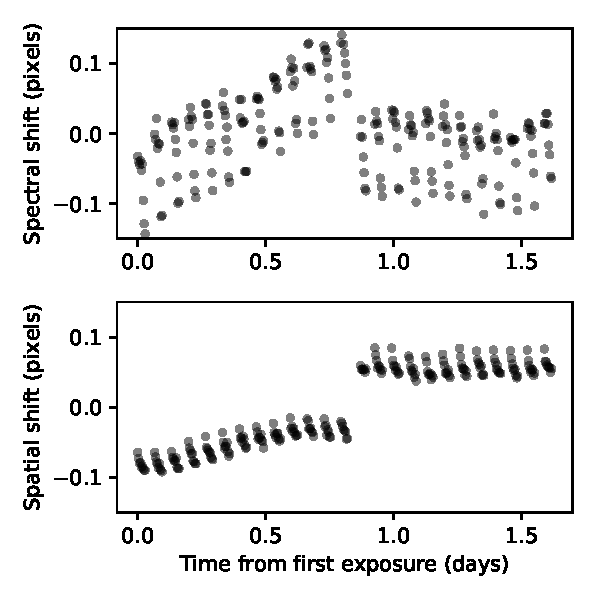
\includegraphics[width = 0.5 \textwidth]{figures/fig4_shifts.pdf}
    \caption{Shift (in pixels) relative to the mean position of the spectrum in the spectral direction (top) and spatial direction (bottom). The largest shift occurs after orbit 14 due to a guide star reacquisition.}
\label{fig:shifts}
\end{figure}

\subsection{Pointing Drift Measurement}
The position of the spectrum on the detector shifts slightly over time ($\sim0.1$ pixel/day) due to the spacecraft's pointing drift. This drift can change the flux measured for the target star: if the spectrum moves onto less sensitive pixels, fewer photoelectrons are recorded. To enable a correction for this effect, we measured the position of the spectrum over time.  

To measure shifts in the spatial direction, we first summed each \texttt{flt} image over all columns (which we dub the ``column sum"). We used the first exposure in the visit as a template, and for each subsequent exposure, we used least-squares minimization to calculate the shift in pixels that minimized the difference between its column sum and the template. The shifts are a fraction of a pixel, so we used the NumPy \texttt{interp} routine to do linear interpolation on a sub-pixel scale. The WFC3 point spread function is undersampled, so we convolved each column sum with a 4-pixel-wide Gaussian  before the interpolation \citep[following][]{deming13}.  

To measure the spectral shifts, we repeated this procedure with two differences: (1) we used the optimally extracted spectrum rather than the column sum; and (2) in addition to calculating the best fit shift, we also calculated a best fit normalization factor (a scalar multiple for the whole spectrum), to ensure that our results are not biased by the varying brightness of the host star during the planet's transit. 

Figure\,\ref{fig:shifts} shows the best fit shifts. Over the entire 26-orbit visit, the maximum shift is less than 0.2 pixel in the spatial direction and 0.3 pixel in the spectral direction. The largest shift occurs after orbit 14, when the telescope reacquired the guide stars. 

\begin{figure}
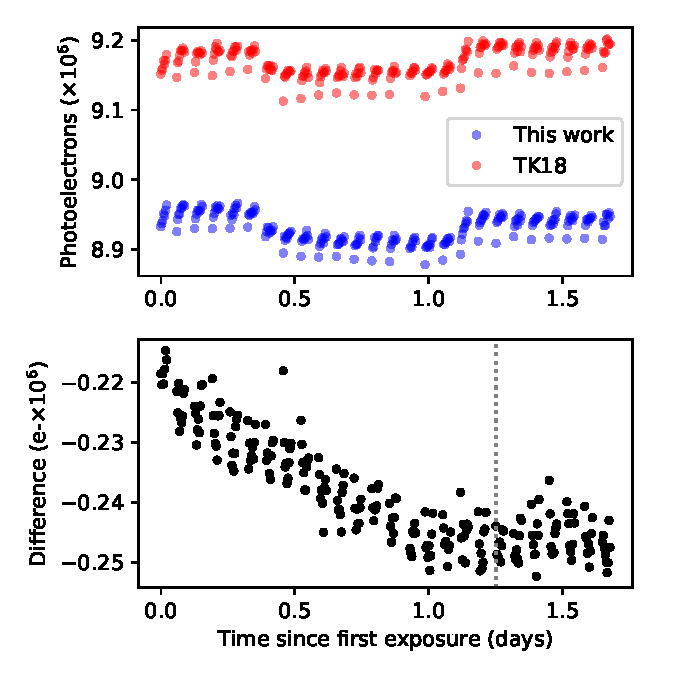
\includegraphics[width = 0.5 \textwidth]{figures/fig6_rawdata.pdf}
    \caption{Top: raw data from this work (blue) compared to TK18 (red). Bottom: the difference in raw photoelectron counts between the data sets. The moon ingress identified by TK18 is marked by the dotted gray line.}
\label{fig:raw}
\end{figure}

\section{Analysis}
The raw light transit light curve (shown in Figure~\ref{fig:raw}) contains both astrophysical signal and instrument systematic noise, which we model simultaneously. 

\subsection{Astrophysics Model}
For the astrophysics, we used the \texttt{planetplanet} package \citep{luger17}, a photodynamical code that calculates light curves for multiple occulting bodies orbiting a star. Within \texttt{planetplanet}, the orbits are computed with the N-body integrator \texttt{REBOUND} \citep{rein12}. The \texttt{planetplanet} model returns the system flux at a specified orbital architecture and time. 

In our analysis, we considered two scenarios: a no-moon model and a moon model. The free parameters for the no-moon model were: the stellar radius $R_*$, the planet radius $R_\mathrm{planet}$, the time of central transit $t_\mathrm{planet}$, and the planet inclination $i$. For the moon model, we added a third body with radius $R_\mathrm{moon}$, transit time $t_\mathrm{moon}$, and orbital period $P_\mathrm{moon}$. We allowed the moon period to vary from 1.6 to 260 days. These limits span the duration of the \HST\ observations (so there is one possible moon occultation event), to the orbit at 0.5 the Hill radius, based on the stability limit for prograde moon orbits \citep{domingos06}. The Hill radius calculation assumed the planet and stellar masses are $1\,M_\mathrm{Jup}$ and $1.37\,M_\odot$.

The models also fixes several parameters that are poorly constrained by the light curve shape. For the moon model, we fixed inclination of the moon to $90^\circ$ to exclude grazing transit scenarios, where the moon radius could be arbitrarily large.  We also fixed the moon mass and eccentricity to zero.  For both the no-moon and moon models, we fixed the planet's orbital period to 287.378949 days \citep{teachey18b}. We also fixed the planet eccentricity to zero and the mass to $1\,M_\mathrm{Jup}$. 

\begin{figure*}
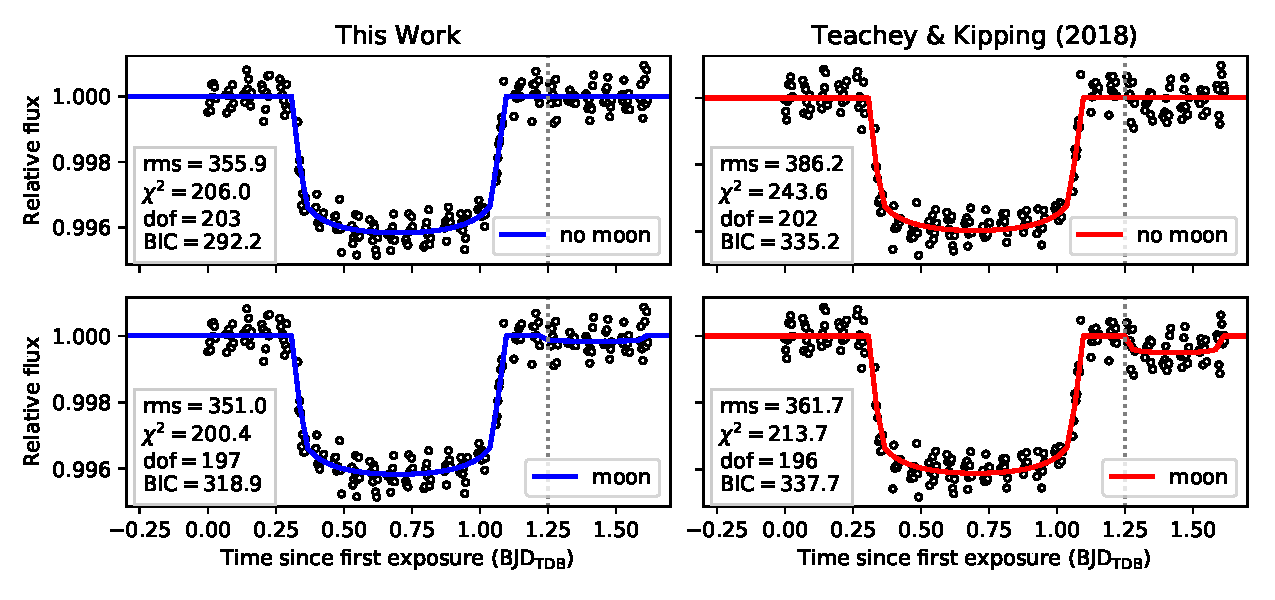
\includegraphics[width = 1.0 \textwidth]{figures/fig3_bestfits.pdf}
    \caption{Best fit models compared to normalized transit light curves from this work (left, blue) and from TK18 (right, red). The top panel shows the best fit no-moon model, and the bottom shows the best fit moon model. The lower left of each panel indicates the fit rms (in ppm), the $\chi_2$, the degrees of freedom, and the change in BIC relative to the lowest value.  Each light curve is divided by its best fit systematics model (XY decorrelation for this work; second-order polynomial and offset for TK18).  The dotted gray line marks the possible moon ingress identified by TK18.}
\label{fig:bestfit}
\end{figure*}


\subsubsection{Stellar Parameters}
For both the moon and no-moon scenarios, we used a quadratic stellar limb darkening law and fixed the coefficients to the prediction for a 5700~K, solar metallicity \texttt{PHOENIX} model from \cite{espinoza15}; $u_1, u_2 = [0.216, 0.183]$.  

We estimated the host star parameters using the Gaia DR2 parallax \citep{Gaia, GaiaDR2} along with UBV photometry from \citet{Everett2012} and JHK photometry from 2MASS \citep{2MASS}. We employed the isochrone python package \citep{isochrone} with the Dartmouth isochrone grid \citep{Dotter2008} to obtain posterior constraints on the stellar parameters. The resulting parameters indicate that Kepler-1625 has stellar mass $1.37^{+0.13}_{-0.16}$ M$_{\odot}$, radius $1.81^{+0.18}_{-0.16}$ R$_{\odot}$, and age $2.8^{+1.6}_{-1.2}$ Gyr. In our analysis, we fixed the stellar mass to the best fit value ($1.37\,M_\odot$), and used a Gaussian prior on the radius, $R_* \sim N(1.81, 0.17)$.


\subsection{Instrument Systematics Model}
There are two systematic trends in the data. One is the orbit-long ramp, attributed to charge traps in the detector filling up over the orbit \citep{zhou17}. The other is a visit-long trend over multiple orbits, which could be due to shifts in the target star position onto more/less sensitive pixels.

To fit the orbit-long ramp, we used the non-parametric model from \cite{teachey18b}, which assigns each of the nine exposures per orbit a normalization constant, $c_1, ..., c_9$. To fit the visit-long trend, we used a linear combination of X and Y position (the shift relative to the mean in the spatial and spectral directions, respectively; shown in Figure~\ref{fig:shifts}).  In sum, for exposure number $i$, the systematics model S is:
\begin{equation}
\label{eq:sys}
    \mathrm{S}_i = c_{j}\times(1 + a\mathrm{X}_i + b\mathrm{Y}_i) 
\end{equation}
where $a$ and $b$, and $c_j$ are free parameters, and $j = i\Mod9 + 1$ is the exposure number relative to the first exposure in the orbit.


\subsection{Light Curve Fits}
We fit the raw, broadband transit light curve using the models described above.  We determined the best fit model parameters with least-squares minimization.  We also ran a Markov chain Monte Carlo (MCMC) fit to determine the posterior probability of each parameters. For the MCMC, we held the ramp parameters $c_1, ..., c_9$ fixed at their best-fit values.  The MCMC used the \texttt{emcee} package \citep{foremanmackey13} with 50 walkers and ran for 5000 steps. We discarded the first 20\% of the MCMC chain as burn-in. As a quick test for convergence, we divided the remainder of the chain in half and confirmed that the results from the first half were consistent with the second half.


\section{Results}
We obtained an excellent fit to the light curve with the no-moon model, as illustrated in  Figure\,\ref{fig:bestfit}. The residuals to our no-moon model fit have rms equal to 362.2 parts per million (ppm), which is within 2\% of the predicted photon shot noise (367 ppm), and yields a $\chi_\nu^2 = 1.05$. The binned rms decreases with the square root of the number of points per bin, as expected for photon noise-limited statistics (see rms versus bin size in Figure~\ref{fig:rms}).

\begin{figure}
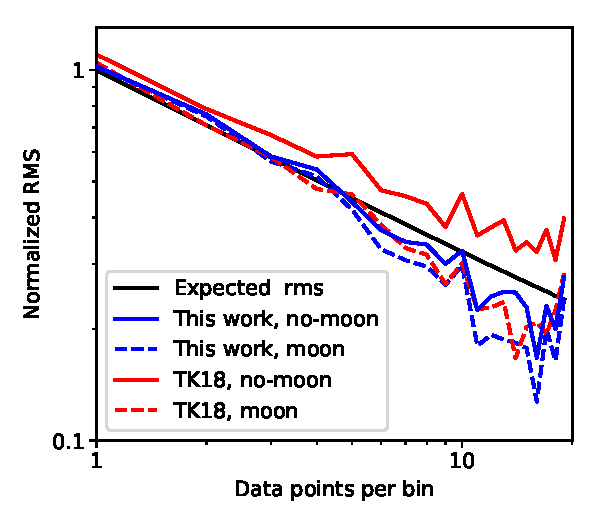
\includegraphics[width = 0.5 \textwidth]{figures/fig2_rms.pdf}
    \caption{Light curve rms versus bin size for the best fit no-moon model. The fit to data from this work (blue line) agrees well with the expected photon-limited, $\sqrt{N}$ decrease in rms with bin size (black line). The TK18 rms (red line) ranges from $1.3 - 2\times$ the photon limit for bin sizes of 1 to 20 data points. The increase in relative rms for larger bin sizes indicates that time-correlated noise is present in the TK18 data.}
\label{fig:rms}
\end{figure}

We also obtained a good fit with the moon model; however, the addition of three more free parameters does not significantly improve the fit quality. The best fit moon model has a radius $r_\mathrm{moon} = 2.4R_\oplus$, a mid-transit time $t_\mathrm{moon} = 2458055.2869\,\mathrm{BJD_{TDB}}$, and a period $P_m = 26.5$ days. This fit has a slightly lower rms than the no-moon model (359.5 ppm versus 362.2 ppm), but the $\chi_\nu^2$ is unchanged (also $1.05$). According to the Bayesian information criterion (BIC), which penalizes unnecessary model complexity, the moon model is disfavored with $\Delta\mathrm{BIC} = 13$. This constitutes strong evidence against the inclusion of a moon \citep{kass95}.  In addition, the moon transit time is not well-constrained by the data. As shown in the posterior distribution in Figure~\ref{fig:corner}, the $2\,\sigma$ confidence interval for the moon's transit includes the entire duration of the observations.  The upper limit on the moon radius is $3.2\,R_\oplus$ at $2\sigma$ confidence and $4.0\,R_\oplus$ at $3\sigma$.

\subsection{Comparison with Teachey \& Kipping (2018)}
\cite{teachey18b} found evidence for the transit of a Neptune-size moon in their analysis of the HST data, in contrast to the findings presented here.  To make a direct comparison with their results, we fit the raw TK18 data directly. 

We fit the data with both the no-moon and models.  For the systematics, we tested the XY decorrelation model described above, but found that it did not perform as well as the systematics models presented in TK18 (10\% higher rms and time-correlated residuals).  We therefore opted to use a TK18 systematics model to enable a fair comparison between our results. We used a second-order polynomial trend in time, a constant offset after orbit 14 (where the guide stars are reacquired), and the non-parameteric orbit-long ramp model. This model has one more free parameter than the systematics model given in Equation~\ref{eq:sys}. Figure\,\ref{fig:bestfit} shows the best fit models.

%Similar to the finding of TK18, the moon model improves the fit quality by a $\Delta\chi^2 = 22.0$. However, even with the moon included, the model does not perform better than our no-moon fit (rms = 363 versus 362 ppm). This differenc

%Overall, we find that the TK18 fits have a larger rms than the fits to our new data reduction. The no-moon model has an rms of 381.5 ppm (compared to 362.2 for our data). 

Similar to the finding of TK18, the moon model improves the fit quality by a $\Delta\chi^2 = 22.0$; however, even with the additional four free parameters, the moon model does not perform better than the no-moon model fit to our data (rms of 363 versus 362 ppm).  This difference in fit quality --- equivalent rms to within 1 ppm, but four additional parameters --- corresponds to $\Delta\mathrm{BIC} = 23.9$, which is strong evidence against the moon.  
%Even when a moon is included, the fit is still slightly worse (rms of 363.4 ppm) than our best no-moon model, in spite of four additional free parameters.  

The moon model also yields qualitatively different posterior distributions for the two data sets.  For the TK18 data, the moon radius and transit time are peaked at $r_\mathrm{moon} = 4.0^{+0.8}_{-0.6}\,R_\oplus$ ($>2.1\,R_\oplus$ at $3\sigma$ confidence), and $t_\mathrm{moon} =  2458056.29^{+0.06}_{-0.04}\,\mathrm{BJD_{TDB}}$ (as shown in Figure\,\ref{fig:corner}). By contrast, the fit to the new data only yields an upper limit on the moon radius of ($4.0\,R_\oplus$ at $3\sigma$ confidence), and the transit time is unconstrained.

%Our results are consistent with those originally published in TK18, including the large improvement in $\chi^2$ when the moon is included ($\Delta\chi^2 = 22.0$). The posterior distribution for 



%We obtain a better fit (a lower $\chi^2$) with the no-moon model fit to our data than we obtain with the moon model fit to the TK18 data, even though it has four additional free parameters.


\begin{figure}
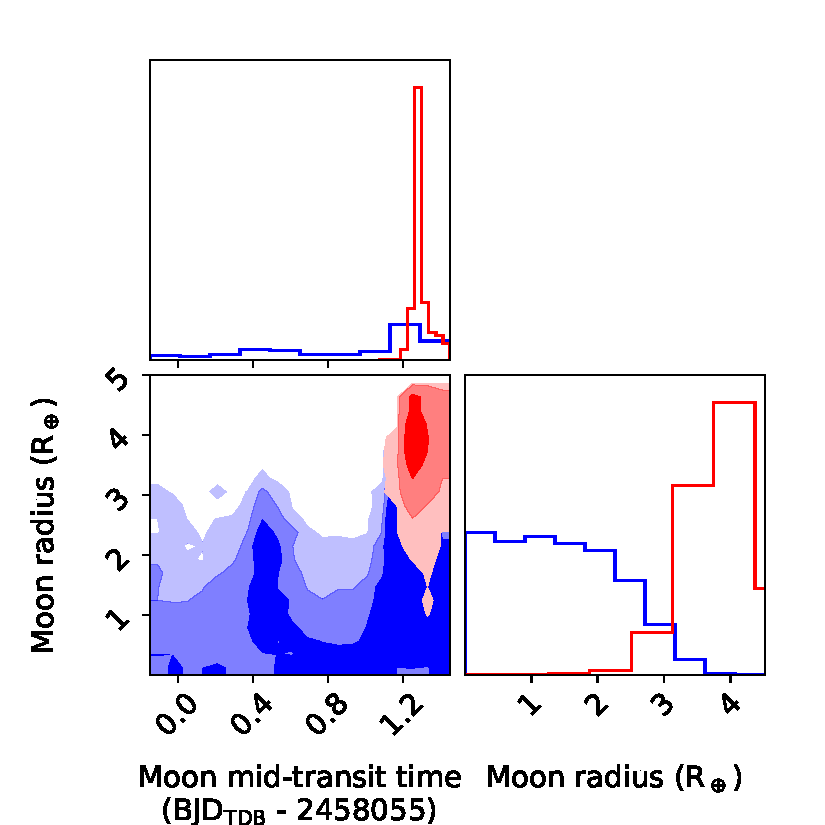
\includegraphics[width = 0.5 \textwidth]{figures/fig5_pairs.pdf}
    \caption{Posterior distributions for the moon radius and time of transit based on an MCMC fit to data from this work (blue) and from TK18 (red). The shading corresponds to $1-$, $2-$, and $3\sigma$ contours (darkest to lightest). These values are marginalized over all other model parameters. The diagonal shows the normalized posterior probability density.}
\label{fig:corner}
\end{figure}

\section{Discussion}
As discussed above, we do not recover the moon. Our analysis was designed to be independent, and as such makes different choices about the data reduction and the choice of sytematics model.

We explored several avenues to determine what caused the difference in our results. We first checked whether the detrending model was responsible. 

We also compared the data directly (see Figure\,\ref{fig:raw}). The data is different!
rotate the image, aperture choice, measurement of the background, outlier masking, 


In this work, we presented an independent analysis of HST observations of the Kepler-1625 system. In contrast to previous analysis by \citep{teachey18b}, we do not find evidence for the transit of a moon. We obtain a better fit to the data without including a moon in the model.  We 



\acknowledgments
The HST data presented in this paper were obtained from the Mikulski Archive for Space Telescopes (MAST). STScI is operated by the Association of Universities for Research in Astronomy, Inc., under NASA contract NAS5-26555. Support for MAST for non-HST data is provided by the NASA Office of Space Science via grant NNX13AC07G and by other grants and contracts.  We also use data from the European Space Agency (ESA) mission {\it Gaia} (\url{https://www.cosmos.esa.int/gaia}), processed by the {\it Gaia} Data Processing and Analysis Consortium (DPAC, \url{https://www.cosmos.esa.int/web/gaia/dpac/consortium}). Funding for the DPAC has been provided by national institutions, in particular the institutions participating in the {\it Gaia} Multilateral Agreement.  We also use data products from the Two Micron All Sky Survey, which is a joint project of the University of Massachusetts and the Infrared Processing and Analysis Center/California Institute of Technology, funded by the National Aeronautics and Space Administration and the National Science Foundation.  This research has made use of the SIMBAD database, operated at CDS, Strasbourg, France; the REBOUND integrator package \citep{rein12}; the NumPy package \citep{van2011numpy}; and NASA's Astrophysics Data System. 


\bibliographystyle{aasjournal}
\bibliography{ms.bib}

\end{document}

% End of file `sample62.tex'.
